\documentclass{standalone}
\usepackage{tikz}
\usetikzlibrary{patterns, positioning}
\usepackage[sfdefault]{ClearSans} %% option 'sfdefault' activates Clear Sans as the default text font
\usepackage[T1]{fontenc}

\begin{document}
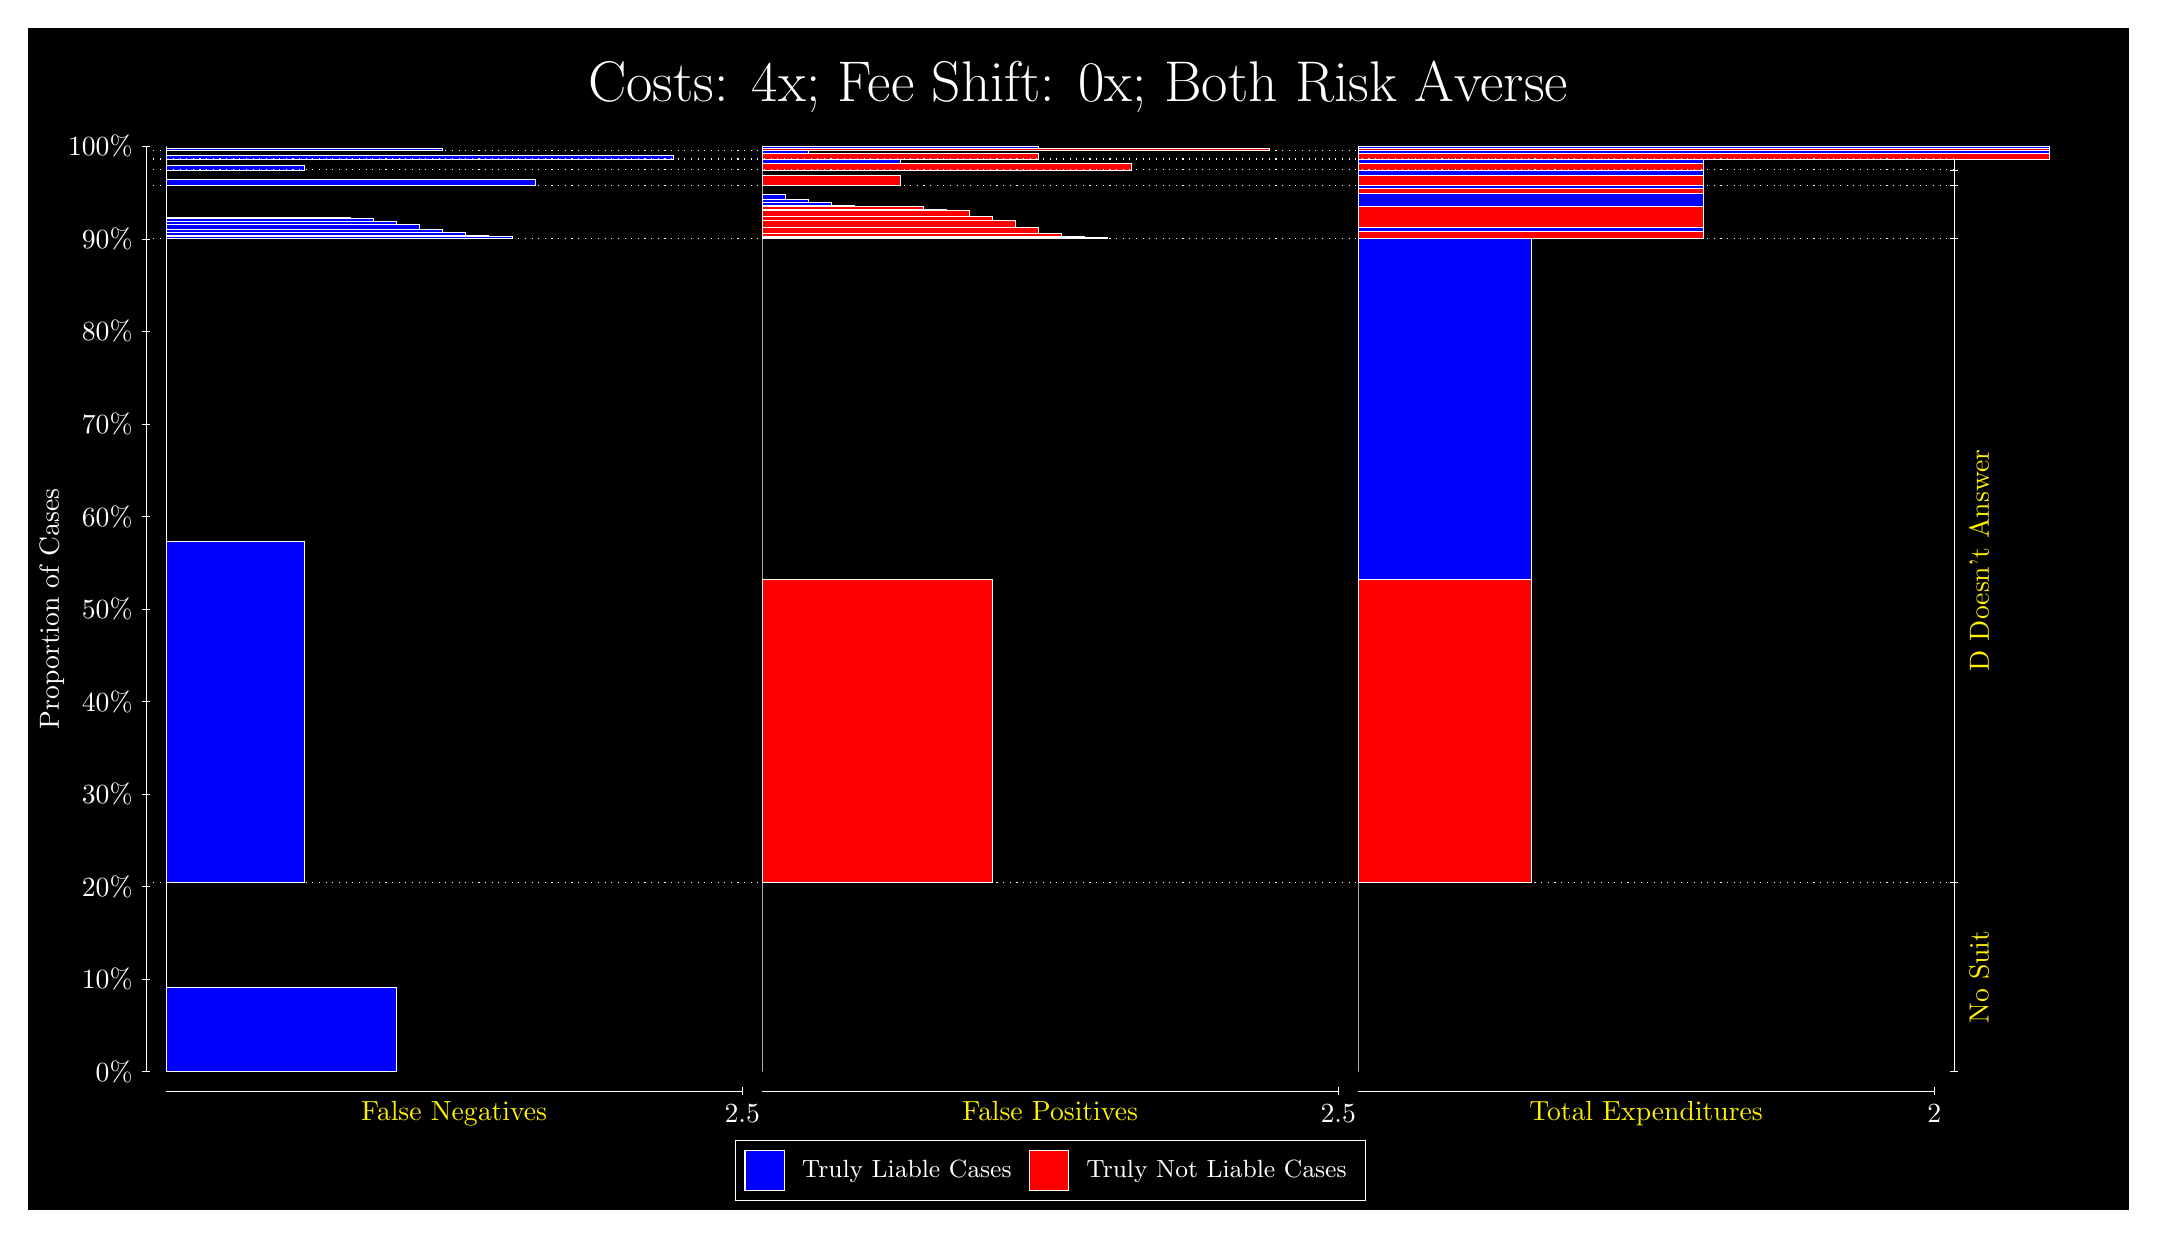
\begin{tikzpicture}
\draw[fill=black] (0,0) rectangle (26.667,15);
\draw[text=white] (0,13.5) rectangle (26.667,15) node[midway] {\huge Costs: 4x; Fee Shift: 0x; Both Risk Averse};
\draw[white, very thin] (1.5,1.75) -- (1.5,13.5);
\node[rotate=90, text=white, anchor=center] at (0.3, 7.625) {Proportion of Cases};
\draw[white, very thin] (1.45,1.75) -- (1.55,1.75);
\node[text=white, anchor=east] at (1.45, 1.75) {0\%};
\draw[white, very thin] (1.45,2.925) -- (1.55,2.925);
\node[text=white, anchor=east] at (1.45, 2.925) {10\%};
\draw[white, very thin] (1.45,4.1) -- (1.55,4.1);
\node[text=white, anchor=east] at (1.45, 4.1) {20\%};
\draw[white, very thin] (1.45,5.275) -- (1.55,5.275);
\node[text=white, anchor=east] at (1.45, 5.275) {30\%};
\draw[white, very thin] (1.45,6.45) -- (1.55,6.45);
\node[text=white, anchor=east] at (1.45, 6.45) {40\%};
\draw[white, very thin] (1.45,7.625) -- (1.55,7.625);
\node[text=white, anchor=east] at (1.45, 7.625) {50\%};
\draw[white, very thin] (1.45,8.8) -- (1.55,8.8);
\node[text=white, anchor=east] at (1.45, 8.8) {60\%};
\draw[white, very thin] (1.45,9.975) -- (1.55,9.975);
\node[text=white, anchor=east] at (1.45, 9.975) {70\%};
\draw[white, very thin] (1.45,11.15) -- (1.55,11.15);
\node[text=white, anchor=east] at (1.45, 11.15) {80\%};
\draw[white, very thin] (1.45,12.325) -- (1.55,12.325);
\node[text=white, anchor=east] at (1.45, 12.325) {90\%};
\draw[white, very thin] (1.45,13.5) -- (1.55,13.5);
\node[text=white, anchor=east] at (1.45, 13.5) {100\%};

\draw[white, very thin] (24.457,1.75) -- (24.457,13.5);
\draw[white, very thin] (24.407,1.75) -- (24.507,1.75);
\node[anchor=west] at (24.407, 1.75) {};
\draw[white, very thin] (24.407,4.1493) -- (24.507,4.1493);
\node[anchor=west] at (24.407, 4.1493) {};
\draw[white, very thin] (24.407,12.332) -- (24.507,12.332);
\node[anchor=west] at (24.407, 12.332) {};
\draw[white, very thin] (24.407,13.006) -- (24.507,13.006);
\node[anchor=west] at (24.407, 13.006) {};
\draw[white, very thin] (24.407,13.202) -- (24.507,13.202);
\node[anchor=west] at (24.407, 13.202) {};
\draw[white, very thin] (24.407,13.339) -- (24.507,13.339);
\node[anchor=west] at (24.407, 13.339) {};
\draw[white, very thin] (24.407,13.452) -- (24.507,13.452);
\node[anchor=west] at (24.407, 13.452) {};
\draw[white, very thin] (24.407,13.5) -- (24.507,13.5);
\node[anchor=west] at (24.407, 13.5) {};

\draw[white, very thin, fill=blue] (1.75,1.75) rectangle (4.6775,2.8204);
\draw[white, very thin, fill=red] (1.75,2.8204) rectangle (1.75,4.1493);
\draw[white, very thin, fill=blue] (1.75,4.1493) rectangle (3.5065,8.4819);
\draw[white, very thin, fill=red] (1.75,8.4819) rectangle (1.75,12.332);
\draw[white, very thin, fill=blue] (1.75,12.332) rectangle (6.1413,12.352);
\draw[white, very thin, fill=blue] (1.75,12.352) rectangle (5.8486,12.365);
\draw[white, very thin, fill=blue] (1.75,12.365) rectangle (5.5558,12.409);
\draw[white, very thin, fill=blue] (1.75,12.409) rectangle (5.2631,12.448);
\draw[white, very thin, fill=blue] (1.75,12.448) rectangle (4.9703,12.506);
\draw[white, very thin, fill=blue] (1.75,12.506) rectangle (4.6775,12.553);
\draw[white, very thin, fill=blue] (1.75,12.553) rectangle (4.3848,12.585);
\draw[white, very thin, fill=blue] (1.75,12.585) rectangle (4.092,12.597);
\draw[white, very thin, fill=blue] (1.75,12.597) rectangle (3.7993,12.604);
\draw[white, very thin, fill=red] (1.75,12.604) rectangle (1.75,13.006);
\draw[white, very thin, fill=blue] (1.75,13.006) rectangle (6.4341,13.078);
\draw[white, very thin, fill=red] (1.75,13.078) rectangle (1.75,13.202);
\draw[white, very thin, fill=blue] (1.75,13.202) rectangle (3.5065,13.261);
\draw[white, very thin, fill=red] (1.75,13.261) rectangle (1.75,13.339);
\draw[white, very thin, fill=blue] (1.75,13.339) rectangle (8.1906,13.382);
\draw[white, very thin, fill=red] (1.75,13.382) rectangle (1.75,13.452);
\draw[white, very thin, fill=blue] (1.75,13.452) rectangle (5.2631,13.477);
\draw[white, very thin, fill=red] (1.75,13.477) rectangle (1.75,13.5);
\draw[white, very thin, fill=red] (9.3189,1.75) rectangle (9.3189,3.0789);
\draw[white, very thin, fill=blue] (9.3189,3.0789) rectangle (9.3189,4.1493);
\draw[white, very thin, fill=red] (9.3189,4.1493) rectangle (12.246,7.9991);
\draw[white, very thin, fill=blue] (9.3189,7.9991) rectangle (9.3189,12.332);
\draw[white, very thin, fill=red] (9.3189,12.332) rectangle (13.71,12.343);
\draw[white, very thin, fill=red] (9.3189,12.343) rectangle (13.417,12.357);
\draw[white, very thin, fill=red] (9.3189,12.357) rectangle (13.125,12.399);
\draw[white, very thin, fill=red] (9.3189,12.399) rectangle (12.832,12.471);
\draw[white, very thin, fill=red] (9.3189,12.471) rectangle (12.539,12.558);
\draw[white, very thin, fill=red] (9.3189,12.558) rectangle (12.246,12.617);
\draw[white, very thin, fill=red] (9.3189,12.617) rectangle (11.954,12.685);
\draw[white, very thin, fill=red] (9.3189,12.685) rectangle (11.661,12.704);
\draw[white, very thin, fill=red] (9.3189,12.704) rectangle (11.368,12.734);
\draw[white, very thin, fill=blue] (9.3189,12.734) rectangle (10.783,12.741);
\draw[white, very thin, fill=blue] (9.3189,12.741) rectangle (10.49,12.753);
\draw[white, very thin, fill=blue] (9.3189,12.753) rectangle (10.197,12.785);
\draw[white, very thin, fill=blue] (9.3189,12.785) rectangle (9.9044,12.832);
\draw[white, very thin, fill=blue] (9.3189,12.832) rectangle (9.6116,12.89);
\draw[white, very thin, fill=blue] (9.3189,12.89) rectangle (9.3189,13.006);
\draw[white, very thin, fill=red] (9.3189,13.006) rectangle (11.075,13.13);
\draw[white, very thin, fill=blue] (9.3189,13.13) rectangle (9.3189,13.202);
\draw[white, very thin, fill=red] (9.3189,13.202) rectangle (14.003,13.279);
\draw[white, very thin, fill=blue] (9.3189,13.279) rectangle (11.075,13.339);
\draw[white, very thin, fill=red] (9.3189,13.339) rectangle (12.832,13.409);
\draw[white, very thin, fill=blue] (9.3189,13.409) rectangle (9.9044,13.452);
\draw[white, very thin, fill=red] (9.3189,13.452) rectangle (15.759,13.475);
\draw[white, very thin, fill=blue] (9.3189,13.475) rectangle (12.832,13.5);
\draw[white, very thin, fill=red] (16.888,1.75) rectangle (16.888,3.0789);
\draw[white, very thin, fill=blue] (16.888,3.0789) rectangle (16.888,4.1493);
\draw[white, very thin, fill=red] (16.888,4.1493) rectangle (19.083,7.9991);
\draw[white, very thin, fill=blue] (16.888,7.9991) rectangle (19.083,12.332);
\draw[white, very thin, fill=red] (16.888,12.332) rectangle (21.279,12.419);
\draw[white, very thin, fill=blue] (16.888,12.419) rectangle (21.279,12.477);
\draw[white, very thin, fill=red] (16.888,12.477) rectangle (21.279,12.736);
\draw[white, very thin, fill=blue] (16.888,12.736) rectangle (21.279,12.907);
\draw[white, very thin, fill=red] (16.888,12.907) rectangle (21.279,12.963);
\draw[white, very thin, fill=blue] (16.888,12.963) rectangle (21.279,13.006);
\draw[white, very thin, fill=red] (16.888,13.006) rectangle (21.279,13.13);
\draw[white, very thin, fill=blue] (16.888,13.13) rectangle (21.279,13.202);
\draw[white, very thin, fill=red] (16.888,13.202) rectangle (21.279,13.279);
\draw[white, very thin, fill=blue] (16.888,13.279) rectangle (21.279,13.339);
\draw[white, very thin, fill=red] (16.888,13.339) rectangle (25.67,13.409);
\draw[white, very thin, fill=blue] (16.888,13.409) rectangle (25.67,13.452);
\draw[white, very thin, fill=red] (16.888,13.452) rectangle (25.67,13.475);
\draw[white, very thin, fill=blue] (16.888,13.475) rectangle (25.67,13.5);
\draw[white, dotted] (1.5,4.1493) -- (24.457,4.1493);
\draw[white, dotted] (1.5,12.332) -- (24.457,12.332);
\draw[white, dotted] (1.5,13.006) -- (24.457,13.006);
\draw[white, dotted] (1.5,13.202) -- (24.457,13.202);
\draw[white, dotted] (1.5,13.339) -- (24.457,13.339);
\draw[white, dotted] (1.5,13.452) -- (24.457,13.452);
\draw[white, very thin] (1.75,1.5) -- (9.0689,1.5);
\node[text=yellow, anchor=north] at (5.4094, 1.5) {False Negatives};
\draw[white, very thin] (9.0689,1.45) -- (9.0689,1.55);
\node[text=white, anchor=north] at (9.0689, 1.45) {2.5};

\draw[white, very thin] (9.3189,1.5) -- (16.638,1.5);
\node[text=yellow, anchor=north] at (12.978, 1.5) {False Positives};
\draw[white, very thin] (16.638,1.45) -- (16.638,1.55);
\node[text=white, anchor=north] at (16.638, 1.45) {2.5};

\draw[white, very thin] (16.888,1.5) -- (24.207,1.5);
\node[text=yellow, anchor=north] at (20.547, 1.5) {Total Expenditures};
\draw[white, very thin] (24.207,1.45) -- (24.207,1.55);
\node[text=white, anchor=north] at (24.207, 1.45) {2};

\node[text=yellow, centered, rotate=90] at (24.777, 2.9496) {No Suit};
\node[text=yellow, centered, rotate=90] at (24.777, 8.2405) {D Doesn't Answer};






\draw (12.978300999999998,1.5) node[draw=none] (baseCoordinate) {};
\begin{scope}[align=center]
        \matrix[scale=0.5, draw=white, below=0.5cm of baseCoordinate, nodes={draw}, column sep=0.1cm]{
            \node[rectangle, draw, minimum width=0.5cm, minimum height=0.5cm, fill=blue] {}; &
            \node[draw=none, font=\small, text=white] (B) {Truly Liable Cases}; &
            \node[rectangle, draw, minimum width=0.5cm, minimum height=0.5cm, fill=red] {}; &
            \node[draw=none, font=\small, text=white] (B) {Truly Not Liable Cases}; \\
            };
\end{scope}

\end{tikzpicture}
\end{document}